\section{Utterance Planning Models}

\begin{frame}{What's the plan at test time?}

   
    \resizebox{\textwidth}{!}{
    \begin{tikzpicture}
   \draw[mLightBrown!30] (6.2,0) -- (6.2,-8.15);
   \draw[mLightBrown!30] (0,0) -- (0,-4.85);

   \uncover<1-2>{
       \node[align=left,text width=10cm,anchor=north west] at (0,0) {\texttt{{\color{mLightBrown}\# Input}\\x = [\\~\\~\\~\\~\\~\\~\\]}};
   }
   \uncover<1-2>{
       \node[anchor=west] at (0.5,-2.8) 
       {\resizebox{5.5cm}{!}{$\pi = \left( \left[\!\!\!\left[ \begin{array}{l}
        \textsc{Inform}\\
        \textrm{\color{Red}name=Aromi}\\
        \textrm{\color{Green}eat\_type=coffee shop}\\
        \textrm{\color{Blue}area=city centre}\\
    \end{array}\right]\!\!\!\right]\right)$ }};


   }
\uncover<1-2>{
    \draw[line width=1.5mm,draw=Green,<->] (5.4,-3.1) to [out=0,in=270] (6.15,-2.8) to [out=90,in=180] (6.8,-2.5);
\node at (4.25,-2.55) {};
    \draw[line width=1.5mm,draw=Red,<->] (4.20,-2.55) to [out=0,in=90] (6.15,-3.10) to [out=270,in=180] (6.70,-6.36);
    \draw[line width=1.5mm,draw=Blue,<->] (4.70,-3.56) to [out=0,in=180] (6.70,-4.36);
}
\uncover<2>{
    \node[color=Green,font=\Huge] at (7.1,-2.5) {\textbf{?}};
    \node[color=Red,font=\Huge] at (7.1,-6.36) {\textbf{?}};
    \node[color=Blue,font=\Huge] at (7.1,-4.36) {\textbf{?}};

   \node[font=\Huge,align=left,anchor=north west] at (8.0, -2) {\textbf{No reference} \\\textbf{utterance} \\\textbf{at test time!}};
}
         \node[align=left,text width=5.75cm,anchor=north west] at (6.2,0) {\texttt{{\color{mLightBrown}\# Output}\\y = [\\ 
                    \uncover<1>{~~~~"<<s>>",}\\ 
                    \uncover<1>{~~~~"for",}\\
                    \uncover<1>{~~~~{{\color{Green}"coffee",}}}\\
                    \uncover<1>{~~~~"in",}\\
                    \uncover<1>{~~~~"the",}\\
                    \uncover<1>{~~~~{\color{Blue}"city",}}\\
                    \uncover<1>{~~~~{\color{Blue}"centre",}}\\
                    \uncover<1>{~~~~",",}\\
                    \uncover<1>{~~~~"try",}\\
                    \uncover<1>{~~~~{\color{Red}"aromi",}}\\
                    \uncover<1>{~~~~".",}\\
                    \uncover<1>{~~~~"<<e>>"}\\
                ] \\ ~
   }};

    \end{tikzpicture}
}
\end{frame}

\begin{frame}{Utterance Planners}

\textbf{Bigram Utterance Planner} (\textsc{BgUP})\\
\begin{itemize}
\item Use training data to esitmate bigram LM over attribute-value sequeunces.\\
~\\
$p(\textit{<<s>>})\times p(\textit{eat\_type=coffee shop}|\textit{<<s>>})\times p(\textit{area=city centre}|\textit{eat\_type=coffee shop})
\times p(\textit{name=Aromi}|\textit{area=city centre})\times
p(\textit{<<e>>}|\textit{name=Aromi})$\\~\\

\item Use constrained beam search to generate a candidate plan from an MR.
\end{itemize}
\end{frame}


\begin{frame}{Utterance Planners}

\textbf{Neural Utterance Planner} (\textsc{NUP})\\
Train a seq2seq model to map:
\begin{center}\vspace{-12pt}\small Increasing Frequency $\rightarrow$ Alignment Training\end{center}

\resizebox{\textwidth}{!}{
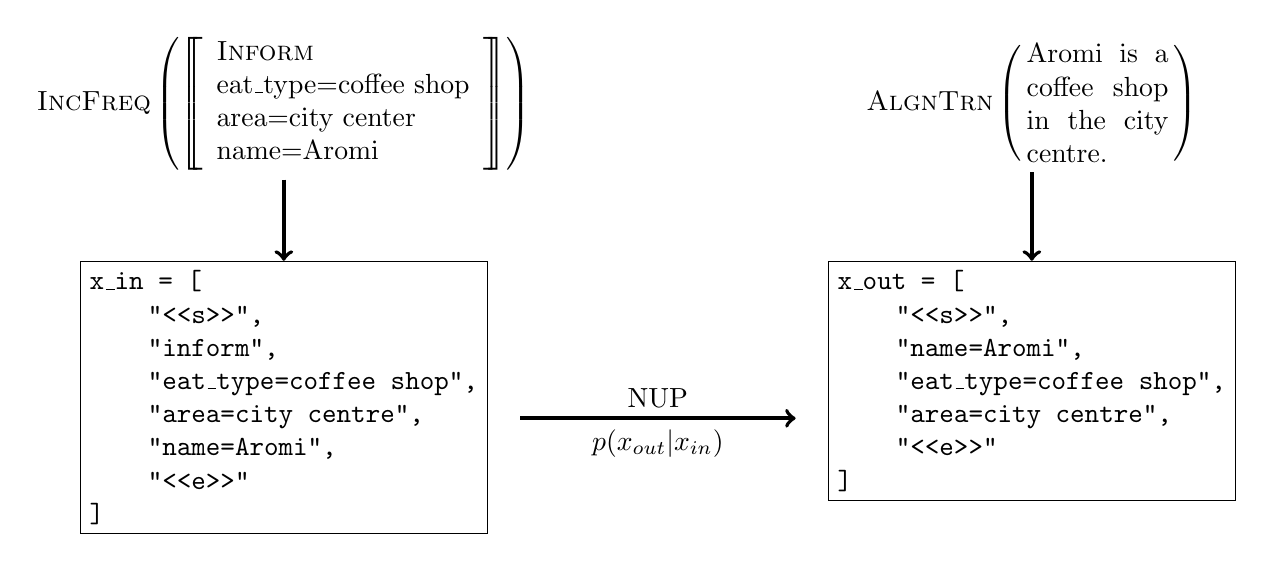
\begin{tikzpicture}
    \node (mr) at (0, 1) {$\textsc{IncFreq}\left(\left[\!\!\!\left[
        \begin{array}{l}
            \textsc{Inform}\\
            \textrm{eat\_type=coffee shop}\\ 
            \textrm{area=city center} \\ 
            \textrm{name=Aromi}
        \end{array}\right]\!\!\!\right]\right)$};
    \node (utt) at (9.5,1) {$\textsc{AlgnTrn}\left(\, {\begin{minipage}{1.8cm}Aromi is a coffee shop in the city centre.\end{minipage}} \,\right)$ };
    \node[align=left,anchor=north,draw] (xin) at (0,-1) {
        \texttt{x\_in = [}\\
            \texttt{~~~~"<<s>>",}\\
            \texttt{~~~~"inform",}\\
            \texttt{~~~~"eat\_type=coffee shop",}\\ 
            \texttt{~~~~"area=city centre",} \\ 
            \texttt{~~~~"name=Aromi",} \\ 
            \texttt{~~~~"<<e>>"}\\
            \texttt{]}};


    \node[align=left,anchor=north,draw] (xout) at (9.5,-1) {
        \texttt{x\_out = [}\\
            \texttt{~~~~"<<s>>",}\\
            \texttt{~~~~"name=Aromi",} \\ 
            \texttt{~~~~"eat\_type=coffee shop",}\\ 
            \texttt{~~~~"area=city centre",} \\ 
            \texttt{~~~~"<<e>>"}\\
            \texttt{]}};

    %\texttt{["<<s>>",\\ "inform",\\ "eat\_type=coffee shop",\\ "area=city centre",\\ "name=Aromi", \\ "<<e>>"]}};

%    \node[align=center] (b) at (0,-4) {\texttt{["<<s>>", "name=Aromi", "eat\_type=coffee shop", "area=city centre", "<<e>>"]}};

%    \draw[line width=0.05cm,->] (a) to (b);
\draw [line width=0.05cm,->] (mr.south) to (xin.north);
\draw [line width=0.05cm,->] (utt.south) to (xout.north);
\draw [line width=0.05cm,->] (3,-3) -- (6.5,-3) node[midway,above] {NUP}
node[midway,below] {$p(x_{out}|x_{in})$};
\end{tikzpicture}
}
\end{frame}

\begin{frame}{Utterance Planners}
    \textbf{Oracle}
    \begin{itemize}
        \item Use Alignment Training ordering obtained from test-set reference utterances.
        \item Assumes clairvoyant knowledge of the test set.
    \end{itemize}

\end{frame}
